%%%%%%%%%%%%%%%%%%%%%%%%%%%%%%%%%%%%
\newcommand{\formalAgentResources}[2]{
	\functionFormal{ar}
	{\setAgents{}{} \times \setRealNumbers{}{}}
	{\setRealNumbersNonNegative{}{}}
}


\begin{figure}
\centering 
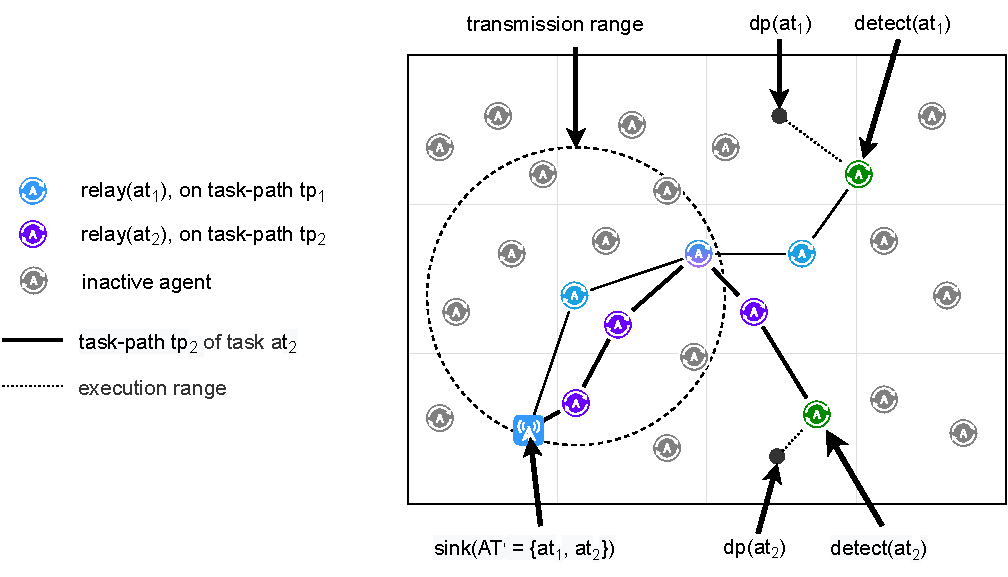
\includegraphics[width=0.9\linewidth]{grid_concept}
\caption[WSN deployment terminology]{WSN deployment terminology}
\label{fig:gridconcept}
\end{figure}

\subsection{Agents, tasks, and resources}

A WSN system is comprised of a set of \textit{agents}, equipped with \textit{sensors}. Tasks are types and can be either \textit{atomic tasks}, for individual measurements, or \textit{composite tasks}, composed of sets of atomic tasks. Composite tasks are allocated from outside the system throughout its lifetime. These composite tasks are then decomposed by agents and the corresponding atomic tasks either completed by that agent, or allocated to other agents to complete or relay to further agents. Completing atomic tasks requires \textit{resources}, such as energy, of which an agent has a fixed amount defined by $\formalAgentResources{}{}$. At at time $\varTime{}{}$, each agent carrying out an atomic task has a certain amount of the resources it possesses $\varResource{}{}$, in this case energy, assigned to completion of tasks of that type, given by $\formalTaskResourceAllocation{}{}$

We can therefore define the system as a tuple $\langle \setAtomicTask{}{}, \setCompositeTask{}{},  \setAgents{}{}, \setResource{}{} \rangle$, where
\begin{itemize}
 \item $\setAtomicTask{}{}$ is a set of atomic tasks where each task is a measurement task performed by a single agent;
 \item $\setCompositeTask{}{} \subseteq \powerSetSymbol{\setAtomicTask{}{}}{}{}$ is the set of composite tasks that occur in the system;
 \item $\setAgents{}{}$ is a set of agents;
 \item $\setResource{}{}$ is a set of resources needed to perform atomic tasks;
\end{itemize}

\subsection{Distribution and location}
The system has a geographical area to monitor defined by a two dimensional grid of real numbers on which agents are distributed randomly such as is common in environmental settings. The \textit{deployment configuration} is a mapping from agents to their respective locations on this grid, $\formalDeployment{}{}$. Each atomic task targets a measurement at a location on this grid, its \textit{demand point} $\functionTaskDemandPoint{}{}$.

\subsection{Node roles and task arcs}
%%%%%%%%%%%%%%%%%%%%%%%%%%%%%%%%%%%%%%%%%%%%
\newcommand{\formalSinkRole}[2]{
	\functionFormal{sink}
	{\setAtomicTask{}{}}
	{\setAgents{}{}}
}
\newcommand{\formalSenseRole}[2]{
	\functionFormal{sense}
	{\setAtomicTask{}{}}
	{\setAgents{}{}}
}
\newcommand{\formalActiveRole}[2]{
	\functionFormal{active}
	{\setAtomicTask{}{}}
	{\powerSetAgents{}{}}
}
\newcommand{\formalIdleRole}[2]{
	\functionFormal{idle_{\setTime{}{}}}
	{\setAtomicTask{}{}}
	{\powerSetAgents{}{}}
}
\newcommand{\formalSleepRole}[2]{
	\functionFormal{sink_{\setTime{}{}}}
	{\setAtomicTask{}{}}
	{\powerSetAgents{}{}}
}
\newcommand{\functionSinkRole}[2]{\functionSignature{sink}{\varAtomicTask{}{}}}
	
\newcommand{\functionSenseRole}[2]{\functionSignature{sense}{\varAtomicTask{}{}}}
\newcommand{\functionActiveRole}[2]{\functionSignature{active_{#1}}{\varAtomicTask{}{}}}
\newcommand{\functionIdleRole}[2]{\functionSignature{idle}{\varAtomicTask{}{}}}
\newcommand{\functionSleepRole}[2]{\functionSignature{sleep}{\varAtomicTask{}{}}}

To simplify discussion of task execution we distinguish agents by the role they play in a given atomic task.
\begin{itemize}
	\item A \textit{sink node} of an atomic task $\varAtomicTask{}{}$ is the agent that first receives the corresponding composite task, and will broadcast the results, $\formalSinkRole{}{}$.
	\item A \textit{sensing node} is the agent that executes the atomic task and so performs the sensor measurement, $\formalSenseRole{}{}$.
	\item An \textit{active node} is an agent that participates in sub-allocating, or routing, that task, but is neither a sink agent nor a sensing agent, $\formalActiveRole{}{}$..
	\item An \textit{idle node} does not participate in the specific task, but does in other tasks in the system during a time period $\setTime{}{}$, $\formalIdleRole{}{}$.
	\item An \textit{sleeping node} does not participate in any of the tasks in the system during a time period $\setTime{}{}$, $\formalSleepRole{}{}$.
\end{itemize}
With these roles in mind, we can now define the  \textit{atomic task arc} as a mapping of atomic tasks to ordered sequence of agents $\formalTaskArc{}{}$ that each atomic task $\varAtomicTask{}{}$ is sub-allocated to. The first agent is the agent that has received the initial composite task, and the last agent is the agent that executes the atomic task, with the sequence of agents in-between relaying the atomic task \footnote{Note, generally communications in WSN networks are multi-hop due to the limited broadcast range of nodes, therefore are $n>0$ active agents sub-allocating the task between the sink and sensing agents.} such that 
$\functionTaskArc{}{} = \lbrace \functionSinkRole{}{}, \functionActiveRole{i}{}, \functionSenseRole{}{} \rbrace_{i=1}^{n}$.

